\chapter{The Hamiltonian Method}
\section{Basics}
\begin{definition}
If the determinant of the matrix 
\begin{align}
a_{ik} = \frac{\partial^2 L(q_m,\dot{q}_m)}{\partial \dot{q}_i \partial \dot{q}_k}
\end{align}
vanishes, the Lagrangian is called degenerate. Otherwise, $L$ is nondegenerate or regular.
\end{definition}
When the Lagrangian is degenerate, some of the velocities $\dot{q}_i$ can disappear when we try to find $p_i(q_i,\dot{q}_i)$. We are left with an equation depending on the coordinates and momenta, called a constraint.
\begin{definition}[Primary constraint]
Equations of the form
\begin{align}
\phi_m(q_i,p_i) = 0, 
\end{align}
where $m = 1, ..., M$ is the number of constraints, are called primary constraints when they follow from the definition of the generalized momentum.
\end{definition}
Let's illustrate what these constraints mean. One can visualize the state of a mechanical system with $n$ degrees of freedom as a point $(q_i,p_i)$ in a $2n$-dimensional phase space ($n$ coordinates and $n$ momenta). The coordinates of this point (the state) depend on time and evolve according to the Hamiltonian equations of motion. 
\begin{figure}[H]
\begin{center}
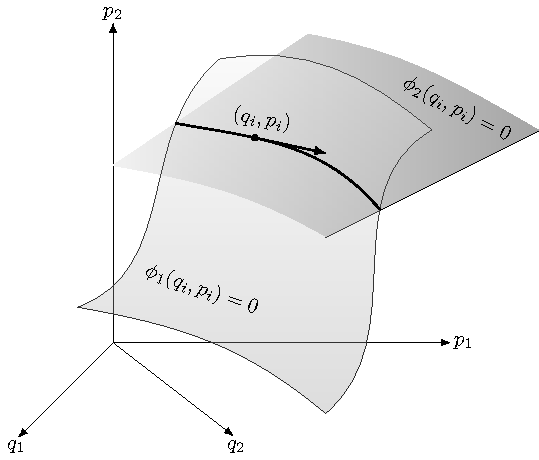
\includegraphics[scale=1.28]{img/constraint.pdf}
\end{center}
\caption{Two intersecting constraint surfaces. The system is only allowed to be in states in which both constraints are fulfilled.}
\label{fig:1}
\end{figure}
In general, the trajectory of this point can fill the whole phase space. When we have constraints, the system is only allowed to be in states in which the constraints are fulfilled. In phase space, they build hypersurfaces on which the point is allowed to move. If every constraint can be fulfilled, the point will move on the intersections of all constraints, like visualized in Fig. \ref{fig:1}. But how to include this into the mathematical formalism? \\
To see, how the constraints enter into the Hamiltonian equations of motion
\begin{align}
\dot{q}_i &= \frac{\partial H}{\partial p_i} \label{eq:1} \\
\dot{p}_i &= - \frac{\partial H}{\partial q_i} \label{eq:2}
\end{align}
and change the dynamics, it will be very useful to write them with Poisson brackets.
\begin{definition}[Poisson bracket]
\begin{align}
\left \{ f(q_i, p_i),g(q_i, p_i) \right \} \equiv \sum_{i=1}^n \left( \frac{\partial f}{\partial q_i} \frac{\partial g}{\partial p_i} - \frac{\partial g}{\partial q_i} \frac{\partial f}{\partial p_i} \right).
\end{align}
\end{definition}
Some properties of the Poisson bracket are:
\begin{enumerate}
\item \(
\begin{aligned}[t]
\left \{ f,g \right \} = - \left \{ g,f \right \}
\end{aligned} \) \ - \ anticommutative
\item \(
\begin{aligned}[t]
\left \{ \alpha f_1 + \beta f_2,g \right \} = \alpha \left \{ f_1,g \right \} + \beta \left \{ f_2,g \right \} 
\end{aligned} \) \ - \ bilinear
\item \(
\begin{aligned}[t]
\left \{  f_1 f_2,g \right \} = f_1 \left \{ f_2,g \right \} + f_2 \left \{ f_1,g \right \} 
\end{aligned} \) \ - \ "derivative"
\item \(
\begin{aligned}[t]
\left \{ \left \{ f,g \right \},h \right \} + \left \{ \left \{ g,h \right \},f \right \} + \left \{ \left \{ h,f \right \},g \right \} = 0 
\end{aligned} \) \ - \ Jacobi identity
\end{enumerate}
These rules hold for any three functions $f,g,h$ of phase space and time (observables).
\begin{theorem}\label{theorem}
The time evolution for any observable $g(q_i,p_i)$ is
\begin{equation}\label{eq:3}
\dot{g} = \frac{dg}{dt} = \left \{ g,H \right \}. 
\end{equation}
It is equivalent to the Hamiltonian equations of motion.
\end{theorem}
\begin{proof}
"$\Rightarrow$" By definition of the total derivative we have
\begin{align}
\frac{dg}{dt} = \sum_{i=1}^n \left( \frac{\partial g}{\partial q_i} \dot{q}_i + \frac{\partial g}{\partial p_i} \dot{p}_i \right) = \sum_{i=1}^n \left( \frac{\partial g}{\partial q_i} \frac{\partial H}{\partial p_i} - \frac{\partial g}{\partial p_i} \frac{\partial H}{\partial q_i} \right) = \left \{ g,H \right \},
\end{align}
where we used the Hamiltonian equations of motion \eqref{eq:1} and \eqref{eq:2}. \\
"$\Leftarrow$" Choose $g = q_k$ and get
\begin{align}
\dot{q}_k = \left \{ q_k,H \right \} = \frac{\partial H}{\partial p_k}.
\end{align}
Analog, with $g = p_k$ we get
\begin{align}
\dot{p}_k = \left \{ p_k,H \right \} = - \frac{\partial H}{\partial q_k}.
\end{align}
\end{proof}
From now on, we will use equation \eqref{eq:3} when we talk about equation of motion. This notation has the big advantage that it can be generalized directly under quantization:
\begin{align}
\left \{ f,g \right \} \  \longrightarrow \ \frac{1}{i \hbar} \ [\hat{f},\hat{g}].
\end{align}
So when we quantize our system and $\hat{g}(\hat{q}_i,\hat{p}_i)$ is an operator, the equation of motion take the form
\begin{align}
\frac{d}{dt}\hat{g} = \frac{i}{\hbar} \ [\hat{H} , \hat{g}],
\end{align}
which is equivalent to the Heisenberg and Schrödinger equation.


\section{From the Lagrangian to the Hamiltonian}
Suppose we have a Lagrangian $L = L(q_i,\dot{q}_i)$. The first step to get the Hamiltonian
\begin{align}
q_i \longrightarrow p_i \equiv \frac{\partial L(q_i,\dot{q}_i)}{\partial \dot{q}_i} = p_i(q_i,\dot{q}_i)
\end{align}
is always possible because one can still differentiate, even when $L$ is degenerate.
For the next step, to express the Hamiltonian only through $q_i$ and $p_i$, it can happen that some velocities $\dot{q}_k$ vanish when we try to calculate the generalized momenta. In this case, it is not possible to express $\dot{q}_k$ through the conjugated momentum $p_k$ and we are left with a primary constraint. So we have not set them by hand, they arised from the definition of the generalized momentum. But there is a nice theorem:
\begin{theorem}
Even if we cannot invert the definition of the generalized momentum and express some velocities through their momenta, 
\begin{align}
H(q_i,\dot{q}_i) = \sum_{i=1}^{n} \dot{q}_i p_i(q_i,\dot{q}_i) - L(q_i,\dot{q}_i), 
\end{align}
is still a function of the coordinates and momenta, all velocities can be eliminated.
\end{theorem}
\begin{proof}
The variation of this function is
\begin{align}
\delta H(q_i,\dot{q}_i) &= \sum_{k=1}^{n} \left( \frac{\partial H}{\partial q_k} \delta q_k + \frac{\partial H}{\partial \dot{q}_k} \delta \dot{q}_k \right) \notag \\
&= \sum_{k=1}^{n} \left( \sum_{i=1}^n \dot{q}_i \frac{\partial p_i}{\partial q_k} - \frac{\partial L}{\partial q_k} \right) \delta q_k + \sum_{k=1}^n \left( p_k + \sum_{i=1}^n \dot{q}_i \frac{\partial p_i}{\partial \dot{q}_k} - \frac{\partial L}{\partial \dot{q}_k} \right) \delta \dot{q}_k \notag \\
&= \sum_{i=1}^{n} \dot{q}_i \left( \sum_{k=1}^n \frac{\partial p_i}{\partial q_k} \delta q_k + \sum_{k=1}^n \frac{\partial p_i}{\partial \dot{q}_k} \delta \dot{q}_k \right) - \sum_{k=1}^n \frac{\partial L}{\partial q_k} \delta q_k \notag \\
&= \sum_{i=1}^n \dot{q}_i \delta p_i - \sum_{i=1}^n \frac{\partial L}{\partial q_i} \delta q_i.
\end{align}
Since we can rewrite the variation in terms of $\delta q_i$ and $\delta p_i$, the Hamiltonian can be expressed as a function of the coordinates and momenta only.
\end{proof}
Comparing the terms in the last line with the variation of $H$ with respect to $\delta q_i$ and $\delta p_i$ and using the Euler-Lagrange-equation, one can find the Hamilton equations of motion. \\
But it is not so easy after all. Remember that we still can have primary constraints $\phi_m$ with vanashing variation:
\begin{align}
\delta \phi_m = 0 = \sum_{i=1}^n \left( \frac{\partial \phi_m}{\partial q_i} \delta q_i + \frac{\partial \phi_m}{\partial p_i} \delta p_i \right).
\end{align}
So we could add this variation to the variation of the Hamiltonian without changing it. This is very useful because normally, $M$ constraints would result in $2n - M$ independent equations of motion but most times, it is easier just to add $M$ independent arbitrary coefficients/functions than reducing the number of equations. So we return the lost degrees of freedom by multiplying our constraints with arbitrary functions $u_m$ and adding them to our variation.
Continuing this idea, since the variation of the constraints is zero, we can add
\begin{align}
0 = \sum_{m=1}^M u_m \delta \phi_m = \sum_{m=1}^M u_m \sum_{i=1}^n \left( \frac{\partial \phi_m}{\partial q_i} \delta q_i + \frac{\partial \phi_m}{\partial p_i} \delta p_i \right)
\end{align}
to 
\begin{align}
\sum_{i=1}^n \left( \frac{\partial H}{\partial p_i} - \dot{q}_i \right) \delta p_i + \sum_{i=1}^n \left( \frac{\partial H}{\partial q_i} + \dot{p}_i \right) \delta q_i = 0,
\end{align}
where we used the Hamilton equations of motion, and get
\begin{align}
\frac{\partial H}{\partial p_i} + \sum_{m=1}^M u_m \frac{\partial \phi_m}{\partial p_i} &= \dot{q}_i \\
\frac{\partial H}{\partial q_i} + \sum_{m=1}^M u_m \frac{\partial \phi_m}{\partial q_i} &= - \dot{p}_i,
\end{align}
which are $2n$ equations with $M$ independent extra-functions. 
It looks like these extra-functions were added to the Hamiltonian, so the following definition is reasonable:
\begin{definition}[Total Hamiltonian]
\begin{align}
H_T(q_i,p_i) \equiv H(q_i,p_i) + \sum_{m=1}^M u_m(q_i,p_i) \phi_m(q_i,p_i).
\end{align}
\end{definition}
Now we want to adapt our results to the formulations of the equations of motion with Poisson brackets. We claim that
\begin{align}
\dot{g} = \left \{ g,H_T \right \} &= \left \{ g,H \right \} + \sum_{m=1}^M u_m  \left \{ g,\phi_m \right \} + \sum_{m=1}^M \left \{ g,u_m \right \} \phi_m \notag \\
&\approx \left \{ g,H \right \} + \sum_{m=1}^M u_m  \left \{ g,\phi_m \right \},
\end{align}
where we have used that all constraints are zero on the constraint surface in the last step. The proof is analog to the proof of Theorem~\ref{theorem}. \\

At this point, we should say something about the usage of constraints and \textit{weak equalities}. First of all, we are not allowed to use the constraints inside a Poisson bracket. We have to calculate the Poisson bracket first and then apply the constraint when it is outside the bracket. If two quantities $f,g$ differ only by a linear combination of constraints, we call them weakly equal (denoted by $f \approx g$). We will use this notation sometimes to distinguish them from usual or strong equations.

\begin{example}
Consider the Lagrangian
\begin{align}
L = L(q,\dot{q}) = q \dot{q} - \frac{q^2}{2}.
\end{align}
From the definition of the generalized momentum follows a primary constraint:
\begin{align}
p = \frac{\partial L}{\partial \dot{q}} = q \ \ \ \Longrightarrow \ \ \ \phi_1 = p - q = 0.
\end{align}
Because of this constraint, the Hamiltonian is not unique:
\begin{align}
H = \dot{q} p - L = \frac{q^2}{2} = \frac{p^2}{2} = \frac{q p}{2}.
\end{align}
This arbitrariness is included in the total Hamiltonian:
\begin{align}
H_T = \frac{q^2}{2} - u_1(q,p) (p-q).
\end{align}
Depending on the choice of $u_1(q,p)$, we can switch from one form to another.
\end{example}

Realizing the appearance of unknown functions in the Hamiltonian and the equations of motion, one might develop bad thoughts about determinism and the predictability of the future.
It turns out that everything keeps predictable and the unknown functions aren't a big problem after all. We will see later that they correspond to mathematical degrees of freedom, so called gauge transformations. \\

For now, let us focus on the consistency of our theory. When we choose the initial conditions, we have to assure ourself that they fulfill the constraints. After time, the equations of motion could lead to a point in phase space which is not on the constraint surface. How to ensure that the system doesn't leave the constraint surface?
Since we want that the primary constraints are fulfilled at every moment, we require
\begin{align}\label{eq:4}
0 \overset{!}{=} \dot{\phi}_k = \left \{ \phi_k,H \right \} + \sum_{m=1}^M u_m  \left \{ \phi_k,\phi_m \right \},
\end{align}
for $k=1,...,M$. This can lead to four cases. First, it could lead directly to an inconsistency saying that the Lagrangian describes no proper system. Second, it could be satisfied identically and we can be sure that everything will be fine. Third, it can lead to an equation that determines the unknown functions and reduces the degrees of gauge freedom. Fourth, it can lead to other constraints, called \textit{secondary constraints}:
\begin{align}\label{eq:5}
0 = \dot{\phi}_1 = \left \{ \phi_1,H \right \} + \sum_{m=1}^M u_m  \left \{ \phi_1,\phi_m \right \} = \left \{ \phi_1,H \right \} = \chi(q,p).
\end{align}
They differ from the primary constraints in the fact that the primary constraints are merely a consequence of the definition of the generalized momenta, while for the secondary constraints, one has to make use of the Lagrangian equations of motion as well. \\
If we have a secondary constraint, then we get another consistency condition because we can work out again $\dot{\chi}$ according to the equation of motion and require that $\dot{\chi} = 0$. This equation has to be treated on the same footing as \eqref{eq:4}. One must again see to which case it leads. If it leads to another secondary constraint, we have to push the process one stage further and check the consistency condition again. \\
We carry on like that until we have exhausted all the consistency conditions, and the final result will be that we are left with a number of secondary constraints together with a number of conditions on the functions $u_m$. The process \footnote{It should be mentioned that it is a controversial topic whether every new constraint should be added to the total Hamiltonian with an undetermined function after each step or not. It only makes a difference when we generate second-class constraints during our procedure. For the most cases, Dirac's procedure (without adding the secondary constraints to the Hamiltonian) works out and leads to the right physics. If one has second-class constraints, one should pay attention and ponder what to do. There are even examples where adding secondary constraints to the Hamiltonian leads to wrong results. That's why we will stick to Dirac and describe his method.} is described in detail by Dirac in his lectures on quantum mechanics \cite{1}. \\

Let's take a closer look on the secondary constraints now. Since they are treated for many purposes like primary constraints, we will denote them like
\begin{align}
\phi_{M+1}(q_i,p_i), ... , \phi_J(q_i,p_i)
\end{align}
and require now 
\begin{align}\label{eq:6}
\dot{\phi}_j = \left \{ \phi_j,H \right \} + \sum_{m=1}^M u_m  \left \{ \phi_j,\phi_m \right \} = 0, 
\end{align}
for $j=1,...,M,M+1,...,J$. These are a number of non-homogeneous linear equations for the unknown functions $u_m$. Let us investigate the solvability of this system. Suppose that we are at the beginning of our procedure and have no secondary constraints yet. Then we can introduce the matrix $\hat{a}$ with components
\begin{align}
a_{jm} = \left \{ \phi_j,\phi_m \right \}, \ \ j,m = 1, \dots, M.
\end{align}
With equation \eqref{eq:6} it follows that
\begin{align}
\sum_{m=1}^M a_{jm} u_m = b_j = - \left \{ \phi_j,H \right \},
\end{align}
which expresses the linear equation system in matrix form. Since the rank of this matrix can be between 0 and $M$:
\begin{align}
0 \leq \text{rank} (\hat{a}) \leq M,
\end{align}
there are two options for solutions of this system. 

\pagebreak

\begin{enumerate}
\item If the rank of the $M \times M$ matrix is maximal, then one has a minimal system of $M$ equations with $M$ variables.
There exists a unique solution 
\begin{align}
u_m = U_m(q_i,p_i).
\end{align}
\item If the rank of the $M \times M$ matrix is $\leq M-1$, then there exist eigenvectors
\begin{align}\label{eq:7}
u_m = U_m(q_i,p_i) + \sum_{a=1}^A v_a(q_i,p_i) V_m^{(a)}(q_i,p_i),
\end{align}
where $A = M - \text{rank} (\hat{a})$ with arbitrary coefficients $v_a$ and any solution $V_m^{(a)}(q_i,p_i)$ of the homogeneous equations. They satisfy 
\begin{align}
\sum_{m=1}^M a_{jm} U_m = b_j \ \ \ \text{and} \ \ \ \sum_{m=1}^M a_{jm} V_m^{(a)} = 0.
\end{align}
The solution is not unique.
\end{enumerate}

Inserting \eqref{eq:7} in the total Hamiltonian, we get
\begin{align}\label{eq:8}
H_T(q_i,p_i) &= H + \sum_{m=1}^M U_m \phi_m + \sum_{a=1}^A v_a \left( \sum_{m=1}^M V_m^{(a)} \phi_m \right) \notag \\
&= H' + \sum_{a=1}^A v_a \tilde{\phi}_a.
\end{align}
Depending on how much the rank of the matrix $\hat{a}$ is smaller than $M$, we are left with $A = M - \text{rank} (\hat{a})$ constraints. So after the procedure, we can find some unknown functions $u_m$ and reduce their degree of freedom in some cases. The general rules are:
\begin{enumerate}
\item If the $u$'s vanish $\longrightarrow$ introduce secondary constraints
\item If not $\longrightarrow$ find conditions on the $u$'s and reduce their degree of freedom.
\end{enumerate}


For the following analysis, we introduce a useful terminology:
\begin{definition}[First-class quantity]
A quantity $R(q_i,p_i)$ is first-class, if it has zero Poisson brackets with all the $\phi$'s:
\begin{align}
\left \{ R,\phi_j \right \} = \sum_{j' = 1}^J r_{j j'} \phi_{j'} \approx 0,
\end{align}
where $j = 1, ... , J$. Otherwise, $R$ is second-class.
\end{definition}
It is important to find all constraints first and then talk about what is first-class and second-class. The following theorem shows a nice property of first-class quantities.

\pagebreak

\begin{theorem}
The Poisson bracket of two first-class quantities is also first-class.
\end{theorem}
\begin{proof}
Let $R,S$ be first-class. Then we have 
\begin{align}
\left \{ R,\phi_j \right \} &= \sum_{j' = 1}^J r_{j j'} \phi_{j'} \approx 0 \\
\left \{ S,\phi_j \right \} &= \sum_{j' = 1}^J s_{j j'} \phi_{j'} \approx 0.
\end{align}
Using the Jacobi identity and the Einstein summation convention, we have
\begin{align}
\left \{ \left \{ R,S \right \},\phi_j \right \} &= \left \{ \left \{ R,\phi_j \right \},S \right \} - \left \{ \left \{ S,\phi_j \right \},R \right \} \notag \\
&= \left \{ r_{j j'} \phi_{j'},S \right \} - \left \{ s_{j j'} \phi_{j'},R \right \} \notag \\
&= r_{j j'} \left \{ \phi_{j'},S \right \} + \left \{ r_{j j'},S \right \} \phi_{j'} - s_{j j'} \left \{ \phi_{j'},R \right \} - \left \{ s_{j j'},R \right \} \phi_{j'} \notag \\
&\approx 0.
\end{align}
\end{proof}

It turns out that our Hamiltonian in equation \eqref{eq:8} is first-class. To see this, check that every term is first-class:
\begin{itemize}
\item \(
\begin{aligned}[t]
\left \{ H',\phi_j \right \} &= \left \{ H + \sum_{m=1}^M U_m \phi_m ,\phi_j \right \} \approx  \left \{ H ,\phi_j \right \} + \sum_{m=1}^M U_m \left \{ \phi_m ,\phi_j \right \} \notag \\
&= b_j - \sum_{m=1}^M a_{jm} U_m = b_j - b_j = 0.
\end{aligned} \)
\item \(
\begin{aligned}[t]
\left \{ v_a \tilde{\phi}_a,\phi_j \right \} \approx v_a \left \{\tilde{\phi}_a,\phi_j \right \} = v_a \sum_{m=1}^M V_m^{(a)} \left \{ \phi_m ,\phi_j \right \} = - v_a \sum_{m=1}^M a_{jm} V_m^{(a)} = 0.
\end{aligned} \)
\end{itemize}


\section{Examples}

Now, we present two typical exersices. Consider the Lagrangian
\begin{align}
L = \frac{1}{2} \left[ \left( \frac{d}{dt} - y \right) x \right]^2 = \frac{1}{2} \left(\dot{x} - xy \right)^2.
\end{align}
First, calculate the conjugate momentum:
\begin{align}
p_x &= \frac{\partial L}{\partial \dot{x}} = \dot{x} - xy \\
p_y &= \frac{\partial L}{\partial \dot{y}} = 0.
\end{align}
From here, we get our first constraint: $\phi_1 = p_y = 0$. \\

The Hamiltonian is given by
\begin{align}
H &= \dot{x} p_x + \dot{y} p_y - \frac{1}{2} \left(\dot{x} - xy \right)^2 \notag \\
&= (p_x + xy)p_x - \frac{1}{2} p_x^2 \notag \\
&= \frac{1}{2} p_x^2 + xy p_x.
\end{align}
But it is not unique. The full Hamiltonian is
\begin{align}
H_T = H + u(x,p_x,y,p_y) \phi_1.
\end{align}
In the following, we will write $u = u(x,p_x,y,p_y)$ but keep in mind that it depends on all these variables. We get the equation of motion by
\begin{align}
\dot{g} = \left \{ g,H \right \} + u \left \{ g,\phi_1 \right \}.
\end{align}
We notice that
\begin{align}
0 = \dot{\phi}_1 = \left \{ \phi_1,H \right \} + u \left \{ \phi_1,\phi_1 \right \} = \left \{ p_y,\frac{1}{2} p_x^2 + xy p_x \right \} = \left \{ p_y,y \right \} x p_x = - x p_x.
\end{align}
Which leads to a secondary constraint:
\begin{align}
\left.
\begin{array}{llll}
      \text{Either:} & x = 0 & \Rightarrow &  p_x = 0 \\
      \text{Or:} & p_x = 0
\end{array}
\right \} \Longrightarrow \phi_2 = p_x = 0.
\end{align}
Let's check whether it satisfies the condition that we required for a constraint: 
\begin{align}
0 \overset{?}{=} \dot{\phi}_2 = \left \{ \phi_2,H \right \} + u \left \{ \phi_2,\phi_1 \right \} = \left \{ p_x,\frac{1}{2} p_x^2 + xy p_x \right \} = \left \{ p_x,x \right \} y p_x = - y p_x \approx 0.
\end{align}
So it is consistent and we get no more constraints. We can also check that $\phi_1, \phi_2$ and $H$ are first-class. We show it only for $H$:
\begin{align}
\left \{ H,\phi_1 \right \} &= \left \{ \frac{1}{2} p_x^2 + xyp_x, p_x \right \} = y p_x \approx 0 \\
\left \{ H,\phi_2 \right \} &= \left \{ \frac{1}{2} p_x^2 + xyp_x, p_y \right \} = x p_x \approx 0.
\end{align}


Another example which is quite similar to string theory, is the following. 
\begin{align}
L = q_1 q_2 (\dot{q}_1 + \dot{q}_2).
\end{align}
Following the procedure, we get two primary constraints:
\begin{align}
p_1 &= \frac{\partial L}{\partial \dot{q}_1} = q_1 q_2 \ \ \ \Longrightarrow \ \ \ \phi_1 = p_1 - q_1 q_2 = 0. \\
p_2 &= \frac{\partial L}{\partial \dot{q}_2} = q_1 q_2 \ \ \ \Longrightarrow \ \ \ \phi_2 = p_2 - q_1 q_2 = 0.
\end{align}
The Hamiltonian is
\begin{align}
H = \dot{q}_1 p_1 + \dot{q}_2 p_2 - q_1 q_2 (\dot{q}_1 + \dot{q}_2) = 0.
\end{align}
At this point, it is useful to notice the following theorem. \\

\begin{theorem}
\label{Theorem}
If the Lagrangian $L$ is homogeneous of degree $1$ in the velocities  
\begin{align}
L(q_i,\lambda \dot{q}_i) = \lambda L(q_i,\dot{q}_i), \label{eq:9}
\end{align}
then $H(q_i,p_i) = 0$.
\end{theorem}
\begin{proof}
The proof of this theorem is analog to the proof of Euler's homogeneous function theorem. 
Differentiating both sides of equation \eqref{eq:9} with respect to $\lambda$ yields
\begin{align}
L(q_i,\dot{q}_i) = \frac{\partial L(q_i,\lambda \dot{q}_i)}{\partial \lambda} = \sum_k \dot{q}_k \frac{\partial L(q_i,\lambda \dot{q}_i)}{\partial (\lambda \dot{q}_k)} .
\end{align}
By setting $\lambda = 1$, we obtain
\begin{align}
\sum_k \dot{q}_k \frac{\partial L(q_i,\dot{q}_i)}{\partial \dot{q}_k} - L(q_i,\dot{q}_i) = H(q_i,p_i) = 0.
\end{align}
\end{proof}

So we didn't even have to calculate the Hamiltonian because our Lagrangian is homogeneous of degree $1$. \\

The total Hamiltonian is
\begin{align}
H_T = 0 + u_1 \phi_1 + u_2 \phi_2
\end{align}
and the equation of motion is
\begin{align}
\dot{g} = u_1 \left \{ g, \phi_1 \right \} + u_2 \left \{ g, \phi_2 \right \}.
\end{align}

With the identity $\{ q_i, p_k \} = \delta_{ik}$, we get $\{ \phi_1 , \phi_2 \} = q_2 - q_1$ and obtain a new (secondary) constraints out of the requirement that
\begin{align}
0 \overset{!}{=} \dot{\phi}_1 &= u_1 \left \{ \phi_1, \phi_1 \right \} + u_2 \left \{ \phi_1, \phi_2 \right \} = u_2 (q_2 - q_1) \\
0 \overset{!}{=} \dot{\phi}_2 &= u_1 \left \{ \phi_2, \phi_1 \right \} + u_2 \left \{ \phi_2, \phi_2 \right \} = u_1 (q_1 - q_2).
\end{align}
\textit{First case $\phi_3 = q_1 - q_2 = 0$.} \\
We have to check that this constraint fulfills our requirement too:
\begin{align}
0 \overset{!}{=} \dot{\phi}_3 &= u_1 \left \{ \phi_3, \phi_1 \right \} + u_2 \left \{ \phi_3, \phi_2 \right \} = u_1 - u_2.
\end{align}
This is just an additional condition on the functions $u_1$ and $u_2$, saying that $u_1 = u_2 = v$. \\

The total Hamiltonian is therefore
\begin{equation}
H_T = v ( \phi_1 + \phi_2 ).
\end{equation}
Now, we want to see whether the Hamiltonian is first-class or second-class. But have we found already all constraints? There is a theorem saying that there is always an even number of second-class constraints, if one cannot combine all secondary constraints to get a new primary constraint. We will proof it later but for now, in our case, we only have one secondary constraint, so we have to find more constraints by combining the old ones:
\begin{align}
\tilde{\phi}_1 &= \phi_1 + \phi_2 = 0 \\
\tilde{\phi}_2 &= \phi_1 - \phi_2 = 0.
\end{align}
And now check which of them are first-class or second-class:
\begin{itemize}
\item \(
\begin{aligned}[t]
\left \{ \tilde{\phi}_1,\tilde{\phi}_2 \right \} = \left \{ p_1 + p_2 - 2 q_1 q_2, p_1 - p_2 \right \} = 2 (q_1 - q_2) = 0.
\end{aligned} \)
\item \(
\begin{aligned}[t]
\left \{ \tilde{\phi}_1,\phi_3 \right \} = \left \{ p_1 + p_2 - 2 q_1 q_2, q_1 - q_2 \right \} = -1 + 1 = 0.
\end{aligned} \)
\item \(
\begin{aligned}[t]
\left \{ \tilde{\phi}_2,\phi_3 \right \} = \left \{ p_1 - p_2, q_1 - q_2 \right \} = -2.
\end{aligned} \)
\end{itemize}
So $\tilde{\phi}_1$, and therefore our Hamiltonian, is first-class and $\tilde{\phi}_2,\phi_3$ are second-class like we expected. We notice:
\begin{definition}
True secondary constraints are secondary constraints which one cannot combine to first-class quantities.
\end{definition}

\textit{Second case $q_1 \neq q_2 \Longrightarrow u_1 = u_2 = 0$.} \\
And the total Hamiltonian is zero.



\section{Gauge Transformations}
In this section, we will see the meaning of the arbitrary coefficients in the total Hamiltonian \eqref{eq:8}.
With the equation of motion, one can express little changes in the function $g$:
\begin{align}\label{eq:10}
\frac{\Delta g}{\Delta t} = \dot{g} = \left \{ g,H' \right \} + \sum_{a=1}^A v_a \left \{ g,\tilde{\phi}_a \right \}.
\end{align}
Since the $v_a$ are arbitrary, there are many possible results for $\Delta g$. The situation is illustrated in Fig.~\ref{fig:2}.

\begin{figure}[H]
\begin{center}
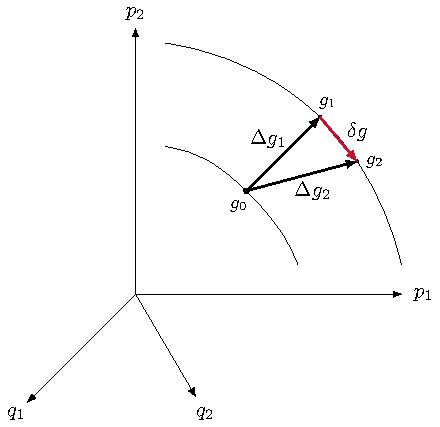
\includegraphics[scale=1.4]{img/gauge1.pdf}
\end{center}
\caption{Evolution of the observable $g$ in phase space.}
\label{fig:2}
\end{figure}

The time evolution of the observable $g$ for small intervals $\Delta t$ can be estimated as
\begin{align}
g(t + \Delta t) = g_0 + \Delta g,
\end{align}
where $\Delta g$ is given by equation \eqref{eq:10}:
\begin{align}
\Delta g = \left \{ g,H' \right \} \Delta t + \sum_{a=1}^A \left( v_a \Delta t \right) \left \{ g,\tilde{\phi}_a \right \}.
\end{align}

Let's choose two different $v_a^{(1)}$ and $v_a^{(2)}$ with which we land eather on $g_1$ or $g_2$, the corresponding change $\Delta g_i$ can be written as:
\begin{align}
\Delta g_1 &= \left \{ g,H' \right \} \Delta t + \sum_{a=1}^A \left( v_a^{(1)} \Delta t \right) \left \{ g,\tilde{\phi}_a \right \} \\
\Delta g_2 &= \left \{ g,H' \right \} \Delta t + \sum_{a=1}^A \left( v_a^{(2)} \Delta t \right) \left \{ g,\tilde{\phi}_a \right \}.
\end{align}

Different functions $v_a^{(i)}$ lead to different results $\Delta g_i$. This means that $g(t + \Delta t)$ is not well defined and depends on the functions $v_a^{(i)}$. The key to the solution of this problem is to say that all \textit{mathematical states} $g_i$ correspond to the same \textit{physical state} $g(t + \Delta t)$. Like in electrodynamics, where $\vec{A} \longrightarrow \vec{A}' = \vec{A} + \nabla f$ leaves the magnetic field unchanged. \\

The transformation which leads from $g_1$ to $g_2$ is called a \textit{gauge transformation}:
\begin{align}
g_1 \longrightarrow g_2 =  g_1 + \delta g.
\end{align}

Let us calculate the explicit form of $\delta g$:
\begin{align}
\delta g = \Delta g_2 - \Delta g_1 = \sum_{a=1}^A \left( v_a^{(2)} - v_a^{(1)} \right) \Delta t \left \{ g,\tilde{\phi}_a \right \} \equiv \sum_{a=1}^A \varepsilon_a \left \{ g,\tilde{\phi}_a \right \},
\end{align}
where $\varepsilon_a$ is a small, arbitrary parameter since $\Delta t$ is small.
\label{sec:gauge_transformations}
We see that this \textit{infinitesimal} change can be expressed as the Poisson bracket of $g$ with the primary constraints. We therefore say that primary constraints are generators of \textit{infinitesimal} gauge transforations. \\
More exactly, the first-class primary constraints are generators of gauge transformation since we started with a first-class total Hamiltonian. Later, we will learn more about the role of first-class quantities for gauge transformations. \\

Before continuing, we would like to illustrate gauge transformations with the following example.
Consider the Lagrangian
\begin{align}
L = \frac{1}{2} (x \dot{x} + y \dot{y})^2.
\end{align}
The definition of the generalized momentum 
\begin{align}
p_x &= \frac{\partial L}{\partial \dot{x}} =  x (x \dot{x} + y \dot{y}) \\
p_y &= \frac{\partial L}{\partial \dot{y}} = y (x \dot{x} + y \dot{y})
\end{align}
leads to the primary constraint
\begin{align}
\phi_1 = p_x y - p_y x = 0.
\end{align}
So again, the Hamiltonian is not unique:
\begin{align}
H &= \dot{x} p_x + \dot{y} p_y - \frac{1}{2} (x \dot{x} + y \dot{y})^2 \notag \\
&= x \dot{x} (x \dot{x} + y \dot{y}) + y \dot{y} (x \dot{x} + y \dot{y}) - \frac{1}{2} (x \dot{x} + y \dot{y})^2 \notag \\
&= (x \dot{x} + y \dot{y})^2 - \frac{1}{2} (x \dot{x} + y \dot{y})^2 \notag \\
&= \frac{1}{2} (x \dot{x} + y \dot{y})^2  \notag \\
&= \frac{p_x^2}{2 x^2} = \frac{p_y^2}{2 y^2} = \frac{p_x p_y}{2 x y}.
\end{align}
We therefore build the total Hamiltonian
\begin{align}
H_T = \frac{p_x^2}{2 x^2} + u_1 (p_x y - p_y x),
\end{align}
where the arbitrariness lies completely in the function $u_1$ now. By choosing $u_1$, one can change between the different variants. The equation of motion is given by
\begin{align}
\dot{g} = \left \{ g,H \right \} + u_1 \left \{ g,\phi_1 \right \}.
\end{align}
Let's check whether the consistency condition holds:
\begin{align}
0 = \dot{\phi}_1 &= \left \{ \phi_1,H \right \} + u_1 \left \{ \phi_1,\phi_1 \right \} = \left \{ p_x y - p_y x,\frac{p_x^2}{2 x^2} \right \} \notag \\
&= \frac{p_x^2 y}{2} \left \{ p_x,\frac{1}{x^2} \right \} - \frac{p_y}{2 x^2} \left \{ x,p_x^2 \right \} \notag \\
&= \frac{p_x^2 y}{2} \left(-(-2) \frac{1}{x^3}\right) - \frac{p_y}{2 x^2} 2 p_x \notag \\
&= \frac{p_x (p_x y - p_y x)}{x^3} \notag \\
&= \frac{p_x \phi_1}{x^3} \approx 0. \ \ \ \surd
\end{align}
So $u_1$ remains arbitrary and we have no secondary constraints. It follows that $\phi_1 = \phi$ is first-class (which is always the case when we only have one constraint) and act as a generator of gauge transformations:
\begin{align}
\Delta g = \varepsilon \left \{ g,\phi \right \}.
\end{align}
Let us insert $\phi$ and see which transformations don't change the physical state of the observables:
\begin{itemize}
\item $\Delta x = \varepsilon \left \{ x,\phi \right \} = \varepsilon \left \{ x,p_x y - p_y x \right \}= \varepsilon y$
\item $\Delta y = \varepsilon \left \{ y,\phi \right \} = - \varepsilon x$
\item $\Delta p_x = \varepsilon \left \{ p_x,\phi \right \} = \varepsilon p_y$
\item $\Delta p_y = \varepsilon \left \{ p_y,\phi \right \} = - \varepsilon p_x$.
\end{itemize}
These transformations do look like the infinitesimal version of rotations in $2$ dimensional space. So let us work out the connection. We will show it for the space part and the momentum is completely analogous.
The equations 
\begin{align}
x' &= x + \varepsilon y \\
y' &= y - \varepsilon x
\end{align}
can be written in matrix form like 
\begin{align}
\bar{r} \ ' = \bar{r} + \varepsilon \hat{\omega} \bar{r},
\end{align}
where
\begin{align}
\bar{r} = 
\begin{pmatrix}
    x \\
    y
\end{pmatrix} \ \ \ \text{and} \ \ \
\hat{\omega} = 
\begin{pmatrix}
    0 & 1 \\
    -1 & 0
\end{pmatrix}.
\end{align}
It follows that
\begin{align}
\Delta \bar{r} = \varepsilon \hat{\omega} \bar{r}.
\end{align}
Redefine the small parameter $\varepsilon \longrightarrow \Delta \alpha$ and solve the differential equation:
\begin{align}
\frac{\Delta \bar{r}}{\Delta \alpha} = \hat{\omega} \bar{r} \ \ \Longrightarrow \ \ \bar{r}(\alpha) = \exp(\hat{\omega} \alpha) \bar{r}(0).
\end{align}
To get a better feeling for what this means, we expand the solution into the Taylor series and note that
\begin{align}
\hat{\omega} = 
\begin{pmatrix}
    0 & 1 \\
    -1 & 0
\end{pmatrix}, \ \
\hat{\omega}^2 = - I, \ \
\hat{\omega}^3 = - \hat{\omega}, \ \
\hat{\omega}^4 = I, \ \
\hat{\omega}^5 = \hat{\omega}, \ \dots .
\end{align}
So 
\begin{align}
\bar{r}(\alpha) &= \left( I + \alpha \hat{\omega} + \frac{\alpha^2 \hat{\omega}^2}{2} + \frac{\alpha^3 \hat{\omega}^3}{3 !} + \frac{\alpha^4 \hat{\omega}^4}{4 !} + \dots  \right) \bar{r}(0) \notag \\
&= \Bigg [  \Big ( \underbrace{1 - \frac{\alpha^2}{2} + \frac{\alpha^4}{4 !} - \dots}_{\Large = \ \cos \alpha} \Big ) I + \Big ( \underbrace{\alpha - \frac{\alpha^3}{3 !} + \frac{\alpha^5}{5 !} - \dots}_{\Large = \ \sin \alpha} \Big ) \hat{\omega} \Bigg ] \bar{r}(0) .
\end{align}
\begin{align}
\Longrightarrow \ 
\begin{pmatrix}
    x' \\
    y'
\end{pmatrix} =
\begin{pmatrix}
    \cos \alpha & \sin \alpha \\
    - \sin \alpha & \cos \alpha
\end{pmatrix}
\begin{pmatrix}
    x \\
    y
\end{pmatrix}.
\end{align}
So our suggestion was right, the gauge transformations are really rotations.
We can illustrate this as follows:
\begin{figure}[H]
\begin{center}
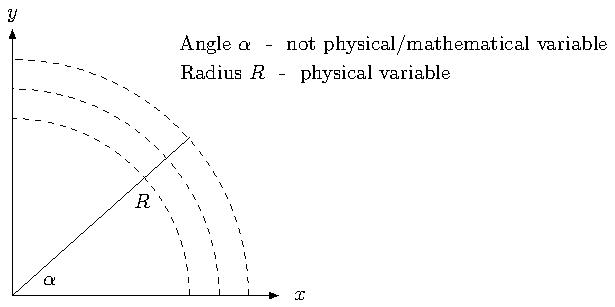
\includegraphics[scale=1.4]{img/rotation.pdf}
\end{center}
\caption{Rotations as gauge transformations.}
\label{fig:3}
\end{figure}
So the quantity 
\begin{align}
R = x^2 + y^2 
\end{align}
will not change under these gauge transformations. To see this, notice that
\begin{align}
\delta R = \varepsilon \left \{ x^2 + y^2 , \phi \right \} = \varepsilon \left \{ x^2 + y^2 , p_x y - p_y x \right \} = \varepsilon (2xy - 2yx) = 0.
\end{align}

With a bit of imagination, one could see this faster. The Lagrangian depends only on the radius $R$, not the angle:
\begin{align}
L = \frac{1}{2} (x \dot{x} + y \dot{y})^2 = \frac{1}{8} \left( \frac{d}{dt} (x^2 + y^2) \right)^2 = \frac{1}{8} \left( \frac{d R^2}{dt} \right)^2 = \frac{1}{8} (2 R \dot{R})^2 = \frac{1}{2} R^2 \dot{R}^2.
\end{align}

\label{sec:finite_gauge_transformations}
How to get from infinitesimal transformations to finite transformations in general? \\

We claim that 
\begin{align}
g(\alpha) = \sum_{n=0}^{\infty} \frac{\alpha^n}{n !} \underbrace{\Large \{ \dots \left \{ \left \{ g_0 , \phi \right \} , \phi \right \} \dots \ , \phi \Large \}}_{n \ \text{times}}
\end{align}
is the general solution.
\begin{proof}
\begin{align}
\frac{d g}{d \alpha} &= \sum_{n=1}^{\infty} \frac{\alpha^{n-1}}{(n-1) !} \underbrace{\Large \{ \dots \left \{ \left \{ g_0 , \phi \right \} , \phi \right \} \dots \ , \phi \Large \}}_{n \ \text{times}} \notag \\
&= \sum_{\bar{n}=0}^{\infty} \frac{\alpha^{\bar{n}}}{\bar{n} !} \underbrace{\Large \{ \dots \left \{ \left \{ g_0 , \phi \right \} , \phi \right \} \dots \ , \phi \Large \}}_{\bar{n} + 1 \ \text{times}} \notag \\
&= \left \{ g , \phi \right \}.
\end{align}
\end{proof}
So, one gets the full transformation out of the constraint $\phi$ by 
\begin{align}\label{eq:11}
g(\alpha) = g_0 + \alpha \left\{ g_0 , \phi \right \} + \frac{\alpha^2}{2} \left \{ \left \{ g_0 , \phi \right \} , \phi \right \} + \dots \ .
\end{align}
With this method we can again derive the same result of the last example:
\begin{itemize}
\item $\left\{ x , \phi \right \} = y$
\item $\left \{ \left\{ x , \phi \right \} , \phi \right \} = \left\{ y , \phi \right \} = - x$
\item $\left \{ \left \{ \left\{ x , \phi \right \} , \phi \right \} , \phi \right \} = \left\{ -x , \phi \right \} = - y$
\item $\left \{ \left \{ \left \{ \left\{ x , \phi \right \} , \phi \right \}, \phi \right \}, \phi \right \} = \left\{ -y , \phi \right \} = x$.
\end{itemize}
So we see that
\begin{align}
x(\alpha) &= \sum_{n=0}^{\infty} \frac{\alpha^n}{n !} \Large \{ \dots \left \{ \left \{ x , \phi \right \} , \phi \right \} \dots \ , \phi \Large \} \notag \\
&= \left( x + \frac{\alpha^2}{2} (-x) + \frac{\alpha^4}{4 !} (x) + \dots \right) + \left( \alpha y + \frac{\alpha^3}{3 !} (-y) + \frac{\alpha^5}{5 !} (y) + \dots \right) \notag \\
&= x \cos \alpha + y \sin \alpha.
\end{align}


\pagebreak

\textbf{General Case} \\

We already know that first-class primary constraints generate gauge transformations, but what about secondary constraints? Will they also be first-class and generate gauge transformations?
Dirac could not show this in general but for all physical situations.

\begin{proof}
Let $\phi_1$ and $\phi_2$ be two constraints.
\begin{figure}[H]
\begin{center}
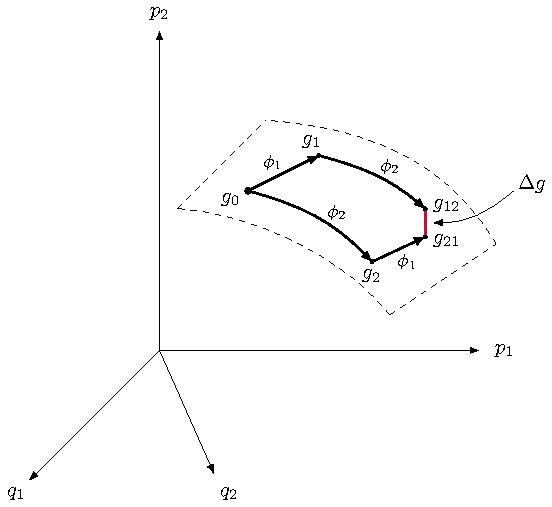
\includegraphics[scale=1.2]{img/gauge2.pdf}
\end{center}
\caption{Different constraints generate different transformations.}
\label{fig:4}
\end{figure}
First, we want to show that transformations between $g_{12}$ and $g_{21}$ are generated by $\left\{ \phi_1 , \phi_2 \right \}$.
We use equation \eqref{eq:11} to the second order to get
\begin{itemize}
\item $g_1 = g_0 + \alpha \left\{ g_0 , \phi_1 \right \} + \frac{\alpha^2}{2} \left \{ \left \{ g_0 , \phi_1 \right \} , \phi_1 \right \} $
\item $g_{12} = g_1 + \beta \left\{ g_1 , \phi_2 \right \} + \frac{\beta^2}{2} \left \{ \left \{ g_1 , \phi_2 \right \} , \phi_2 \right \}  $
\item $g_2 = g_0 + \beta \left\{ g_0 , \phi_2 \right \} + \frac{\beta^2}{2} \left \{ \left \{ g_0 , \phi_2 \right \} , \phi_2 \right \} $
\item $g_{21} = g_2 + \alpha \left\{ g_2 , \phi_1 \right \} + \frac{\alpha^2}{2} \left \{ \left \{ g_2 , \phi_1 \right \} , \phi_1 \right \} .$ 
\end{itemize}
So 
\begin{align}
\Delta g = g_{12} - g_{21} = \dots  = \alpha \beta \left \{ g_0 , \left \{ \phi_1 , \phi_2 \right \} \right \}.
\end{align}
When secondary constraints are first-class then this works out and $\left \{ \phi_1 , \phi_2 \right \}$ is a generator. 

\pagebreak

Now, we want to show that $\left\{ H , \phi_a \right \}$ is also a generator of gauge transformations. 

\begin{figure}[H]
\begin{center}
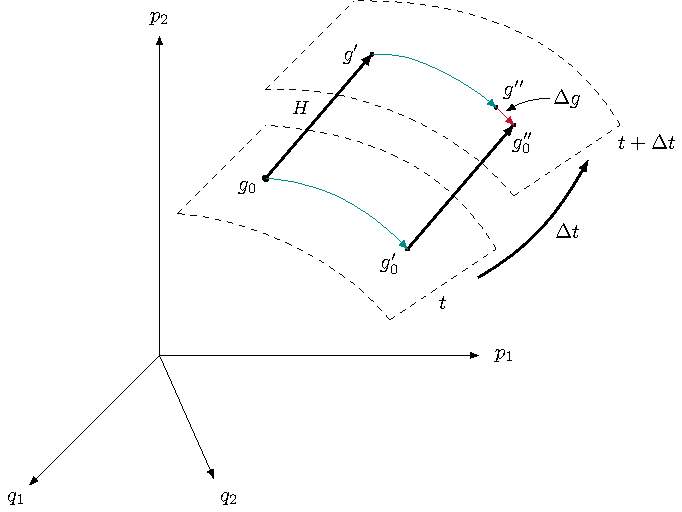
\includegraphics[scale=1.1]{img/gauge3.pdf}
\end{center}
\caption{Physical and mathematical changes of the quantity $g_0$.}
\label{fig:5}
\end{figure}
Consider again
\begin{align}
\frac{\Delta g}{\Delta t} = \left\{ g , H' \right \} + \sum_{a=1}^A v_a \left\{ g , \phi_a \right \}.
\end{align}
We can analyse which part is responsible for which action:
\begin{align}
g' = g(t + \Delta t) = g_0 + \underbrace{\left\{ g_0 , H' \right \} \Delta t}_{\begin{subarray}{l}\text{corresponds to a}\\ \text{physical change}\\
    \text{from layer \ $t \ \rightarrow \ t + \Delta t$.}\end{subarray}}
+ \underbrace{\sum_{a=1}^A \varepsilon_a \left\{ g_0 , \phi_a \right \}}_{\begin{subarray}{2}\text{corresponds to a shift}\\
    \text{within a layer of constant time,}\\
    \text{not physical change.}\end{subarray}}.
\end{align}
Performing a gauge transformation on $g'$ yields:
\begin{align}
g'' = g' + \varepsilon_a \left\{ g' , \phi_a \right \} = g_0 + \left\{ g_0 , H' \right \} \Delta t + 2 \varepsilon_a \left\{ g_0 , \phi_a \right \} + \varepsilon_a \left\{ \left\{ g_0 , H' \right \} \Delta t, \phi_a \right\}.
\end{align}
Now, perform a gauge transformation first
\begin{align}
g_0' = g_0 + \varepsilon_a \left\{ g_0 , \phi_a \right \}
\end{align}
and then calculate the physical change
\begin{align}
g_0'' &= g_0' + \left\{ g_0' , H' \right \} \Delta t + \varepsilon_a \left\{ g_0' , \phi_a \right \} \notag \\
&= g_0 + \left\{ g_0 , H' \right \} \Delta t + 2 \varepsilon_a \left\{ g_0 , \phi_a \right \} + \varepsilon_a \left\{ \left\{ g_0 , \phi_a \right \} , H' \right \} \Delta t.
\end{align}
The difference is 
\begin{align}
\Delta g = g'' - g_0'' &= \varepsilon_a  \left\{ \left\{ g_0 , H' \right \} , \phi_a \right \} \Delta t - \varepsilon_a  \left\{ \left\{ g_0 , \phi_a \right \} , H' \right \} \Delta t \notag \\
&= \varepsilon_a \left\{ g_0 ,  \left\{  H' , \phi_a \right \} \right \} \Delta t ,
\end{align}
which shows that $\left\{  H' , \phi_a \right \}$ is a generator. Both $H'$ and $\phi_a$ are first-class.
\end{proof}

Now that we showed that all first-class quantities generate some kind of gauge transformations, it is reasonable to introduce the following definitions:
\begin{definition}[Total Hamiltonian]
\begin{align}
H_T = H + \sum {\begin{subarray}{l}\text{primary constraints}\\ \text{(first-class)}\end{subarray}}.
\end{align}
\end{definition}

\begin{definition}[Generalized Hamiltonian]
\begin{align}
H_E = H_T + \sum {\begin{subarray}{l}\text{secondary constraints}\\ \text{(first-class)}\end{subarray}}.
\end{align}
\end{definition}

The following example shows a case where all constraints are first-class:
\begin{example}
\begin{align}
L = \frac{1}{2} (\dot{x} - xy)^2
\end{align}
From the definition of the generalized momentum we get the primary constraint
\begin{align}
\phi_1 = p_y = 0
\end{align}
and a secondary constraint from the consistency condition:
\begin{align}
0 = \dot{\phi}_1 \ \ \ \Longrightarrow \ \ \ \phi_2 = p_x = 0.
\end{align}
There are no more constraints. Since both constraints are first-class, we can write the generalized Hamiltonian 
\begin{align}
H_E &= \frac{p_x^2}{2} + xy p_x + v p_y + V p_x \notag \\
&= v p_y + \tilde{V} p_x.
\end{align}
The first constraint $\phi_1 = p_y = 0$ lead to gauge transformations of the form
\begin{align}
\delta y = \varepsilon_1 \left \{ y, p_y \right \} = \varepsilon_1 \\
y \ \longrightarrow \ y' = y + \varepsilon_1
\end{align}
and the second constraint $\phi_2 = p_x = 0$ analogous
\begin{align}
\delta x = \varepsilon_2 \left \{ x, p_x \right \} = \varepsilon_2 \\
x \ \longrightarrow \ x' = x + \varepsilon_2.
\end{align}
\end{example}

\pagebreak

\section{Quantization}

In this section we want to discuss which problems can occur when we try to quantize a Hamiltonian system with constraints.
We will focus on the canonical quantization where we replace every physical observable with an operator and change the Poisson bracket into the commutator:

\begin{align}
q_i \ \longrightarrow \ \hat{q}_i \ \ \ , \ \ \ p_i \ \longrightarrow \ \hat{p}_i.
\end{align}
\begin{align}
\left \{ q_i , p_k \right \} = \delta_{ik} \ \ \longrightarrow \ \ \frac{1}{i \hbar} \left[ \hat{q}_i ,\hat{p}_k \right] = \delta_{ik}.
\end{align}
\begin{align}
\forall g \rightarrow \hat{g} : \ \ \frac{d}{dt} \hat{g} = \frac{1}{i \hbar} \left[ \hat{g} ,\hat{H} \right]  \ \ \Longrightarrow \ \ \hat{H} \psi(q_1, \dots, q_n) = E \psi(q_1, \dots, q_n).
\end{align}

What happens with the constraints? 

They are also replaced by operators and if we act on a wavefunction $\psi$, they will vanish since they vanish on the constraint surface. For first-class constraints this leads to the vanishing of the commutator on the constraint surface:
\begin{align}
\left.
\begin{array}{l}
\hat{\phi}_b \hat{\phi}_a \psi(q_1, \dots, q_n) = 0 \\
\hat{\phi}_a \hat{\phi}_b \psi(q_1, \dots, q_n) = 0
\end{array} \ \right \} \ \
\Longrightarrow \ \ \left[ \hat{\phi}_a ,\hat{\phi}_b \right] \psi = 0.
\end{align}
So for first-class constraints, we can make the transition
\begin{align}
\left \{ \phi_a ,\phi_b \right \} = 0 \ \ \longrightarrow \ \ \left[ \hat{\phi}_a ,\hat{\phi}_b \right] = 0
\end{align}
without problems. 
But if we have second-class constraints, for instance
\begin{align}
\left.
\begin{array}{l}
\chi_1 = q_1 = 0 \\
\chi_2 = p_1 = 0
\end{array} \ \right \} \ \
\Longrightarrow \ \ \left \{ \chi_1 ,\chi_2 \right \} = 1,
\end{align}
it won't work that way and will lead to contradictions:
\begin{align}
\left.
\begin{array}{l}
\hat{p}_1 \hat{q}_1 \psi(q_1, \dots, q_n) = 0 \\
\hat{q}_1 \hat{p}_1 \psi(q_1, \dots, q_n) = 0
\end{array} \ \right \} \ \
\Longrightarrow \ \ \underbrace{\left[ \hat{q}_1 ,\hat{p}_1 \right]}_{= i \hbar} \psi = 0 \ \ \Longrightarrow \ \ \psi = 0.
\end{align}

We can do calculations with the commutator of first-class constraints but not of second-class constraints. 
\begin{align}
H_E = H' + \underbrace{\sum_{a=1}^A v_a \  \tilde{\phi}_a}_{\begin{subarray}{l}\text{primary constraints}\\ \text{(first-class)}\end{subarray}} + \underbrace{\sum v_b \ \tilde{\tilde{\phi}}_b}_{\begin{subarray}{l}\text{secondary constraints}\\ \text{(first-class)}\end{subarray}}.
\end{align}
First-class constraints are generators of gauge transforations and don't change the physical state.
The commutator shows that they are problems with second-class constraints. Let us see how to quantize a Hamiltonian system with second-class constraints. 

\pagebreak

First, we will show that there is always an even number of true second-class constraints (which one cannot combine to first-class constraints). This is good, since every two second-class constraints will lead to a reduction of one degree of freedom.
Mathematically, we will replace the Poisson bracket with the Dirac bracket (which is a generalized Poisson bracket) to fix the problem of second-class constraints.

\label{sec:number_secondary_constraints}
\begin{theorem}
Let $\chi_1, \chi_2, \dots, \chi_S$ be true second-class constraints. Then $S$ is even.
\end{theorem}
%komischer abstand hier ...
\begin{proof}
Introduce the  matrix
\begin{align}
\hat{a}_{ik} = \left \{ \chi_i , \chi_k \right \}, \ \ \ 1 \leq i,k \leq S,
\end{align}
which is obviously antisymmetric because of the antisymmetry of the Poisson bracket. Since the determinant of an odd dimensional antisymmetric matrix is automatically zero, we have to show that $\det (\hat{a}) \neq 0$ which would imply that $S$ is even. \\
Suppose $S$ is odd and $\det (\hat{a}) = 0$. Then $\text{rank}(\hat{a}) = T < S$. \\
Find a minor of $\hat{a}$ which has $\text{rank} = T$ and $\det \neq 0$ and build the \\ $(T+1) \times (T+1)$ - matrix
\begin{align}
\hat{b} =
\left( 
\arraycolsep=1.4pt\def\arraystretch{1.4}
\begin{array}{c|cccc}
\chi_1 & \left\{ \chi_1,\chi_{k_1} \right\} & \left\{ \chi_1,\chi_{k_2} \right\} & \cdots & \left\{ \chi_1,\chi_{k_T} \right\} \\
\chi_2 & \left\{ \chi_2,\chi_{k_1} \right\} & \left\{ \chi_2,\chi_{k_2} \right\} & \cdots & \left\{ \chi_2,\chi_{k_T} \right\} \\
\vdots & \vdots & \vdots & \ddots & \vdots \\
\chi_T & \left\{ \chi_T,\chi_{k_1} \right\} & \left\{ \chi_T,\chi_{k_2} \right\} & \cdots & \left\{ \chi_T,\chi_{k_T} \right\} \\ \cline{1-5}
\chi_{T+1} & \left\{ \chi_{T+1},\chi_{k_1} \right\} & \left\{ \chi_{T+1},\chi_{k_2} \right\} & \cdots & \left\{ \chi_{T+1},\chi_{k_T} \right\} 
\end{array} \right),
\end{align}
where $\chi_{T+1}$ is an arbitrary constraint which is left. We claim that $\det (\hat{b})$ is first-class. This would lead to a contradiction since we can't reach a first-class quantity with true second-class constraints.
Let's show this: \\
\begin{align}
\left\{ \det (\hat{b}),\phi_j \right\} &= 
\det \left( 
\arraycolsep=1.4pt\def\arraystretch{1.4}
\begin{array}{c|cccc}
\left\{ \chi_1,\phi_j \right\} & \left\{ \chi_1,\chi_{k_1} \right\} & \left\{ \chi_1,\chi_{k_2} \right\} & \cdots & \left\{ \chi_1,\chi_{k_T} \right\} \\
\left\{ \chi_2,\phi_j \right\} & \left\{ \chi_2,\chi_{k_1} \right\} & \left\{ \chi_2,\chi_{k_2} \right\} & \cdots & \left\{ \chi_2,\chi_{k_T} \right\} \\
\vdots & \vdots & \vdots & \ddots & \vdots \\
\left\{ \chi_T,\phi_j \right\} & \left\{ \chi_T,\chi_{k_1} \right\} & \left\{ \chi_T,\chi_{k_2} \right\} & \cdots & \left\{ \chi_T,\chi_{k_T} \right\} \\
\left\{ \chi_{T+1},\phi_j \right\} & \left\{ \chi_{T+1},\chi_{k_1} \right\} & \left\{ \chi_{T+1},\chi_{k_2} \right\} & \cdots & \left\{ \chi_{T+1},\chi_{k_T} \right\} 
\end{array} \right) \notag \\[14pt] 
&+ 
\det \left( 
\arraycolsep=1.4pt\def\arraystretch{1.4}
\begin{array}{c|c|ccc}
\chi_1 & \left\{ \left\{ \chi_1,\chi_{k_1} \right\},\phi_j \right\} & \left\{ \chi_1,\chi_{k_2} \right\} & \cdots & \left\{ \chi_1,\chi_{k_T} \right\} \\
\chi_2 & \left\{ \left\{ \chi_2,\chi_{k_1} \right\},\phi_j \right\} & \left\{ \chi_2,\chi_{k_2} \right\} & \cdots & \left\{ \chi_2,\chi_{k_T} \right\} \\
\vdots & \vdots & \vdots & \ddots & \vdots \\
\chi_T & \left\{ \left\{ \chi_T,\chi_{k_1} \right\},\phi_j \right\} & \left\{ \chi_T,\chi_{k_2} \right\} & \cdots & \left\{ \chi_T,\chi_{k_T} \right\} \\
\chi_{T+1} & \left\{ \left\{ \chi_{T+1},\chi_{k_1} \right\},\phi_j \right\} & \left\{ \chi_{T+1},\chi_{k_2} \right\} & \cdots & \left\{ \chi_{T+1},\chi_{k_T} \right\} 
\end{array} \right) \notag \\[14pt] 
&+ \dots \ .
\end{align}
Only the first term is really interesting because we can Laplace expand every other term with respect to the first column and use the fact that $\chi_1, \chi_2, \dots, \chi_{T+1}$ vanish on the constraint surface. \\

Now, there can be several cases: 
\begin{itemize}
\item If $\phi_j$ is first-class, then the Poisson brackets $\left\{ \chi_i,\phi_j \right\}$ will vanish and we are done.
\item If $\phi_j$ is second-class, then it is one of $\chi_1, \dots, \chi_S$ and there are two options:
\begin{enumerate}
\item $\phi_j \in \{ \chi_{k_1}, \dots, \chi_{k_T} \}$, then there will be two equal columns $\Rightarrow \det =0$.
\item $\phi_j \in \{ \chi_{k_{T+1}}, \dots, \chi_{k_S} \}$, then the matrix will be a $(T+1) \times (T+1)$ - minor of the matrix $\hat{a}$ but we fixed $\text{rank} (\hat{a}) = T$, so again $\det = 0$.
\end{enumerate}
\end{itemize}
We showed that $\left\{ \det (\hat{b}),\phi_j \right\} = 0, \ \forall \phi_j$. \\
$\Longrightarrow  \det (\hat{b})$ is a first-class quantity.
\end{proof}

For being able to quantize a Hamiltonian system with second-class constraints, Dirac invented the Dirac bracket:
\label{sec:dirac_bracket}

\begin{definition}[Generalized Dirac bracket]
\begin{align}
\left\{ f,g \right\}_D = \left\{ f,g \right\} - \sum_{i,j = 1}^S \left\{ f,\chi_i \right\} (\hat{a}^{-1})_{ij} \left\{ \chi_j,g \right\}.
\end{align}
\end{definition}

The Dirac bracket has all the properties of the Poisson bracket $+$ fixes the problems:
\begin{enumerate}
\item \(
\begin{aligned}[t]
\left \{ f,g \right \}_D = - \left \{ g,f \right \}_D
\end{aligned} \) \ - \ anticommutative
\item \(
\begin{aligned}[t]
\left \{ \alpha f_1 + \beta f_2,g \right \}_D = \alpha \left \{ f_1,g \right \}_D + \beta \left \{ f_2,g \right \}_D 
\end{aligned} \) \ - \ bilinear
\item \(
\begin{aligned}[t]
\left \{  f_1 f_2,g \right \}_D = f_1 \left \{ f_2,g \right \}_D + f_2 \left \{ f_1,g \right \}_D 
\end{aligned} \) \ - \ "derivative"
\item \(
\begin{aligned}[t]
\left \{ \left \{ f,g \right \}_D,h \right \}_D + \left \{ \left \{ g,h \right \}_D,f \right \}_D + \left \{ \left \{ h,f \right \}_D,g \right \}_D = 0 
\end{aligned} \) \ - \ Jacobi identity
\end{enumerate}

Moreover the equation of motion doesn't change:
\begin{align}
\dot{g} = \left \{ g,H_T \right \}_D = \left \{ g,H_T \right \}
\end{align}
because $H_T$ is a first-class quantity.
The advantage is that every quantity is first-class with the Dirac bracket because the second-class constraints turn to first-class constraints:
\begin{align}
\left \{ g, \chi_j \right \}_D &= \left\{ g,\chi_j \right\} - \sum_{i,k = 1}^S \left\{ g,\chi_i \right\} (\hat{a}^{-1})_{ij} \left\{ \chi_k,\chi_j \right\} \notag \\
&= \left\{ g,\chi_j \right\} - \sum_{i,k = 1}^S \left\{ g,\chi_i \right\} \delta_{ij} \notag \\
&= 0.
\end{align}
In the last section, we said that we have to find all constraints before classifying them. But with the proofed theorem in mind, we don't have to do it anymore since every constraint will be first-class. 

\pagebreak

The following example shows how every two (initially) second-class constraints reduce the degree of freedom by one.

\begin{example}
Consider two second-class constraints:
\begin{align}
\chi_1 &= q_1 = 0 \\
\chi_2 &= p_1 = 0
\end{align}
Then the Dirac bracket is just
\begin{align}
\left \{ f,g \right \}_D &= \left \{ f,g \right \} - \sum_{i,j = 1}^2 \left\{ f,\chi_i \right\} (\hat{a}^{-1})_{ij} \left\{ \chi_j,g \right\} \notag \\
&= \left \{ f,g \right \} - \left\{ f,\chi_1 \right\} (\hat{a}^{-1})_{12} \left\{ \chi_2,g \right\} - \left\{ f,\chi_2 \right\} (\hat{a}^{-1})_{21} \left\{ \chi_1,g \right\} \notag \\
&= \sum_{i=1}^n \left( \frac{\partial f}{\partial q_i} \frac{\partial g}{\partial p_i} - \frac{\partial g}{\partial q_i} \frac{\partial f}{\partial p_i} \right) - \left( - \frac{\partial f}{\partial p_1} \right) (-1) \left( - \frac{\partial g}{\partial q_1} \right) - \left( \frac{\partial f}{\partial q_1} \right) (+1) \left( \frac{\partial g}{\partial p_1} \right) \notag \\
&= \sum_{i=2}^n \left( \frac{\partial f}{\partial q_i} \frac{\partial g}{\partial p_i} - \frac{\partial g}{\partial q_i} \frac{\partial f}{\partial p_i} \right).
\end{align}
\end{example}

Since there is always an even number of true second-class constraints, the Dirac bracket will always reduce to the normal Poisson bracket with fewer degrees of freedom.